

\subsection{Input Adapter}
The ClimateInputAdapter is a specialized learnable preprocessing module designed to bridge the structural gap between multi-parameter atmospheric grids and the fixed input requirements of the Segment Anything Model (SAM). Since SAM is natively optimized for three-channel RGB imagery, this adapter compresses the 16 atmospheric variables from the ClimateNet dataset into a pseudo-RGB representation that preserves critical geophysical features. 

As depicted in Figure \ref{fig:input_adapter}, the architecture follows a bottleneck convolutional design. It initiates with a 3x3 Conv2d layer to capture local spatial dependencies, followed by sequential 1x1 convolutions that reduce the feature dimensionality from 32 to 16, and ultimately to 3 channels. The module incorporates BatchNorm2d and ReLU activations for internal stabilization. A final Sigmoid activation function constrains the output values to a [0, 1] range, which are subsequently rescaled by 255.0 to align with the standard pixel intensity expected by the SAM image encoder.
\vspace{-1em}
\begin{figure}[!h]
    \centering
    % 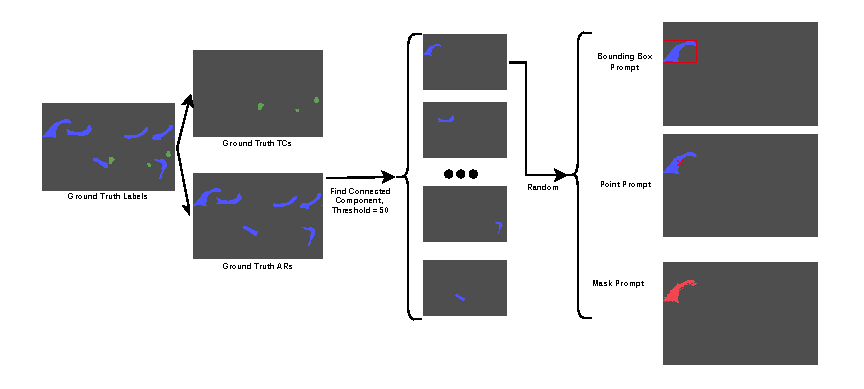
\includegraphics[width=1\textwidth]{graphics/approach/prompt_pipeline-1.pdf}
    \makebox[\textwidth][c]{%
    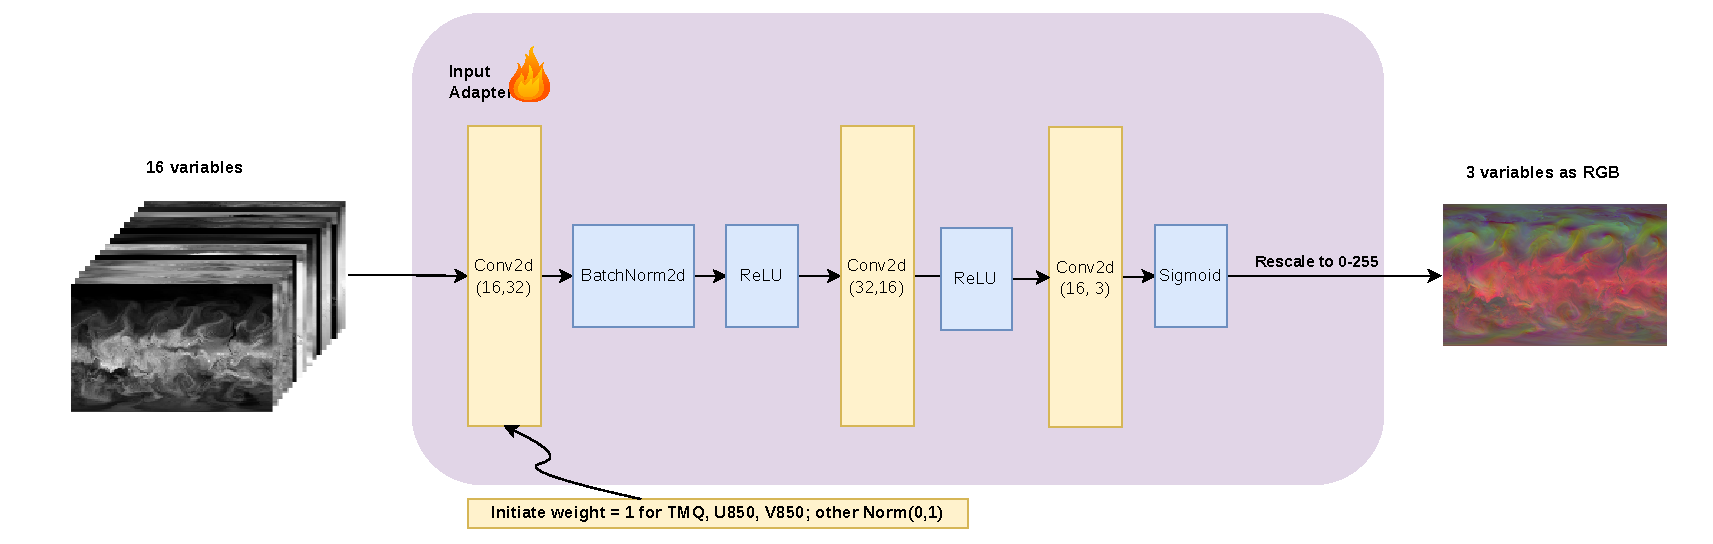
\includegraphics[width=1.3\textwidth]{graphics/approach/input_adapter.pdf}
}
\vspace{-1em}
    \caption{Input Adapter Architecture}
    \label{fig:input_adapter}
\end{figure}


To maintain physical grounding during the Adaptation Phase, the adapter employs an expert-knowledge initialization strategy. The weights for the most diagnostic variables TMQ, U850, V850, and PSL \cite{radke2024explaining} are set to 1.0 at the center of the convolution kernels. This initialization enables the model to prioritize the point-shaped extrema characteristic of Tropical Cyclones and the elongated moisture corridors of Atmospheric Rivers from the onset of training.
\subsection{Encoder Adapter}

\subsubsection{Learnable Token-based approach}

\begin{figure}[!h]
    \centering
    \begin{minipage}[b]{0.45\textwidth}
        \centering
        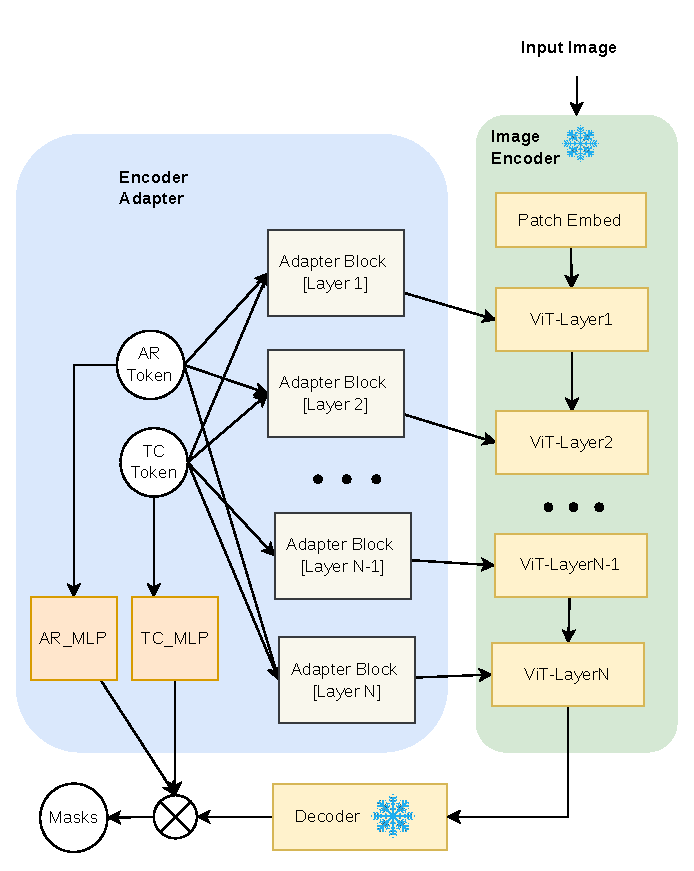
\includegraphics[width=\textwidth]{graphics/approach/token_based_overview.pdf}
        \caption{Overview}
    \end{minipage}
    \hfill
    \begin{minipage}[b]{0.45\textwidth}
        \centering
        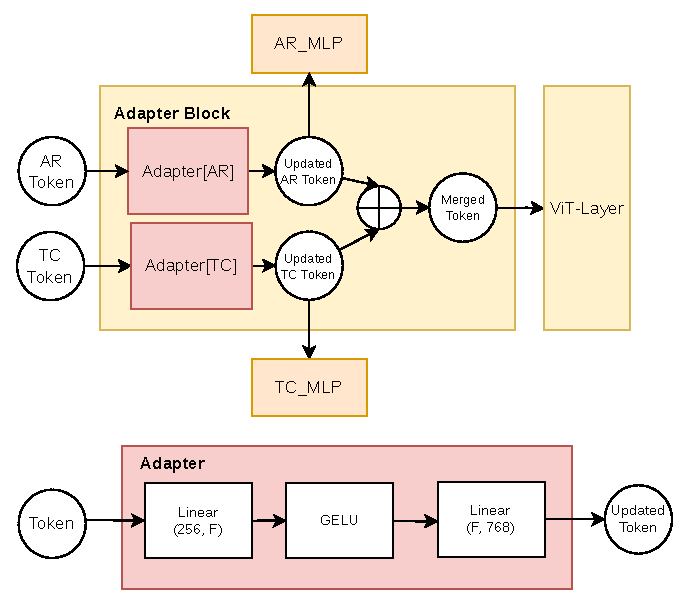
\includegraphics[width=\textwidth]{graphics/approach/token_based_detail.pdf}
        \caption{Detail}
    \end{minipage}
    \caption{Token-based approach architecture}
    \label{fig:token_architecture}
\end{figure}

\subsubsection{LoRA approach}
To adapt SAM to interpret multi-parameter atmospheric grids, we apply LoRA adapters to each layer of the Vision Transformer (ViT) encoder \cite{wu2025multi, zhang2024improving}. This "surgeon" approach specifically targets the Query ($q$), Key ($k$), and Value ($v$) projection layers within the multi-head self-attention mechanism, as these layers are critical for capturing the spatial relationships of complex weather phenomena. Mathematically, for an input feature $x \in \mathbb{R}^{1 \times d}$, the adapted forward pass for a given projection is expressed as:
\begin{equation}
h = W_{0}x + \Delta Wx = W_{0}x + BAx
\end{equation}
where $W_0$ is the frozen pre-trained weight, and $B \in \mathbb{R}^{d \times r}$ and $A \in \mathbb{R}^{r \times d}$ are the learnable low-rank matrices \cite{zhu2024melo, wu2025multi}. We initialize matrix $A$ with a Kaiming uniform distribution and matrix $B$ to zero so that the initial state of the model is identical to the original SAM. At the output stage, we introduce two specialized mask decoders with learnable parameters to handle the distinct morphological characteristics of the target classes:

\begin{itemize}
    \item \textbf{TC Decoder}: Optimized for the distinct circular structures of Tropical Cyclones, addressing a severe 257:1 background-to-foreground ratio.
    \item \textbf{AR Decoder}: Tailored for the narrow, "ribbon-like" corridors of Atmospheric Rivers, which present a more moderate 17:1 class imbalance.
\end{itemize}

This dual-decoder design allows the model to learn class-specific localization priors and structural discovery independently for each meteorological feature.

% \ifdefined\pdfobjcompresslevel
%   \pdfobjcompresslevel=0
% \fi
% \ifdefined\pdfvariable
%   \pdfvariable objcompresslevel=0
% \fi

\begin{figure}[!h]
    \centering
    \begin{minipage}[b]{0.5\textwidth}
        \centering
        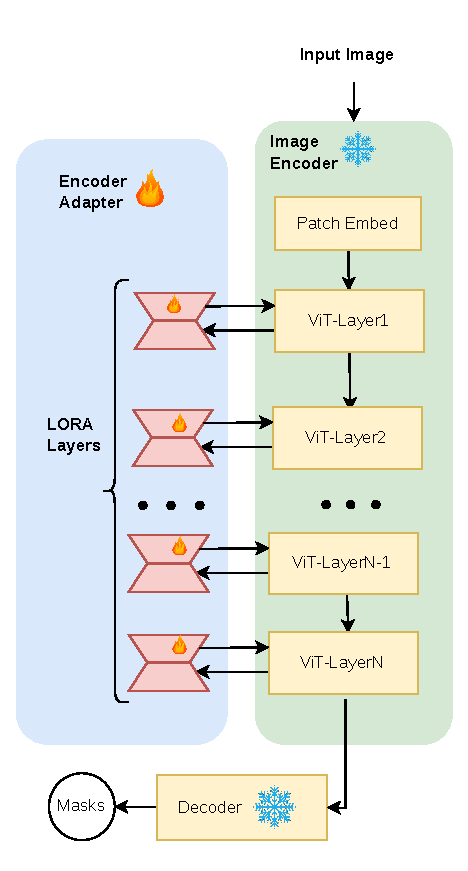
\includegraphics[width=\textwidth]{graphics/approach/lora_overview.pdf}
        \caption{Overview}
    \end{minipage}
    \hfill
    \begin{minipage}[b]{0.45\textwidth}
        \centering
        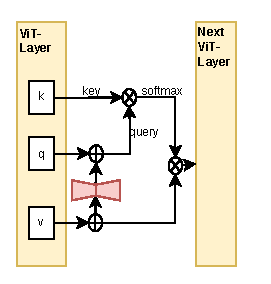
\includegraphics[width=\textwidth]{graphics/approach/lora_detail.pdf}
        \caption{Detail}
    \end{minipage}
    \caption{LoRA adaptation architecture}
    \label{fig:lora_architecture}
\end{figure}

\subsection{Automatic Prompt Generator}

\subsubsection{CGNet}

\subsubsection{Multi-scale Fusion}

\begin{figure}[!h]
    \centering
    \makebox[\textwidth][c]{%
        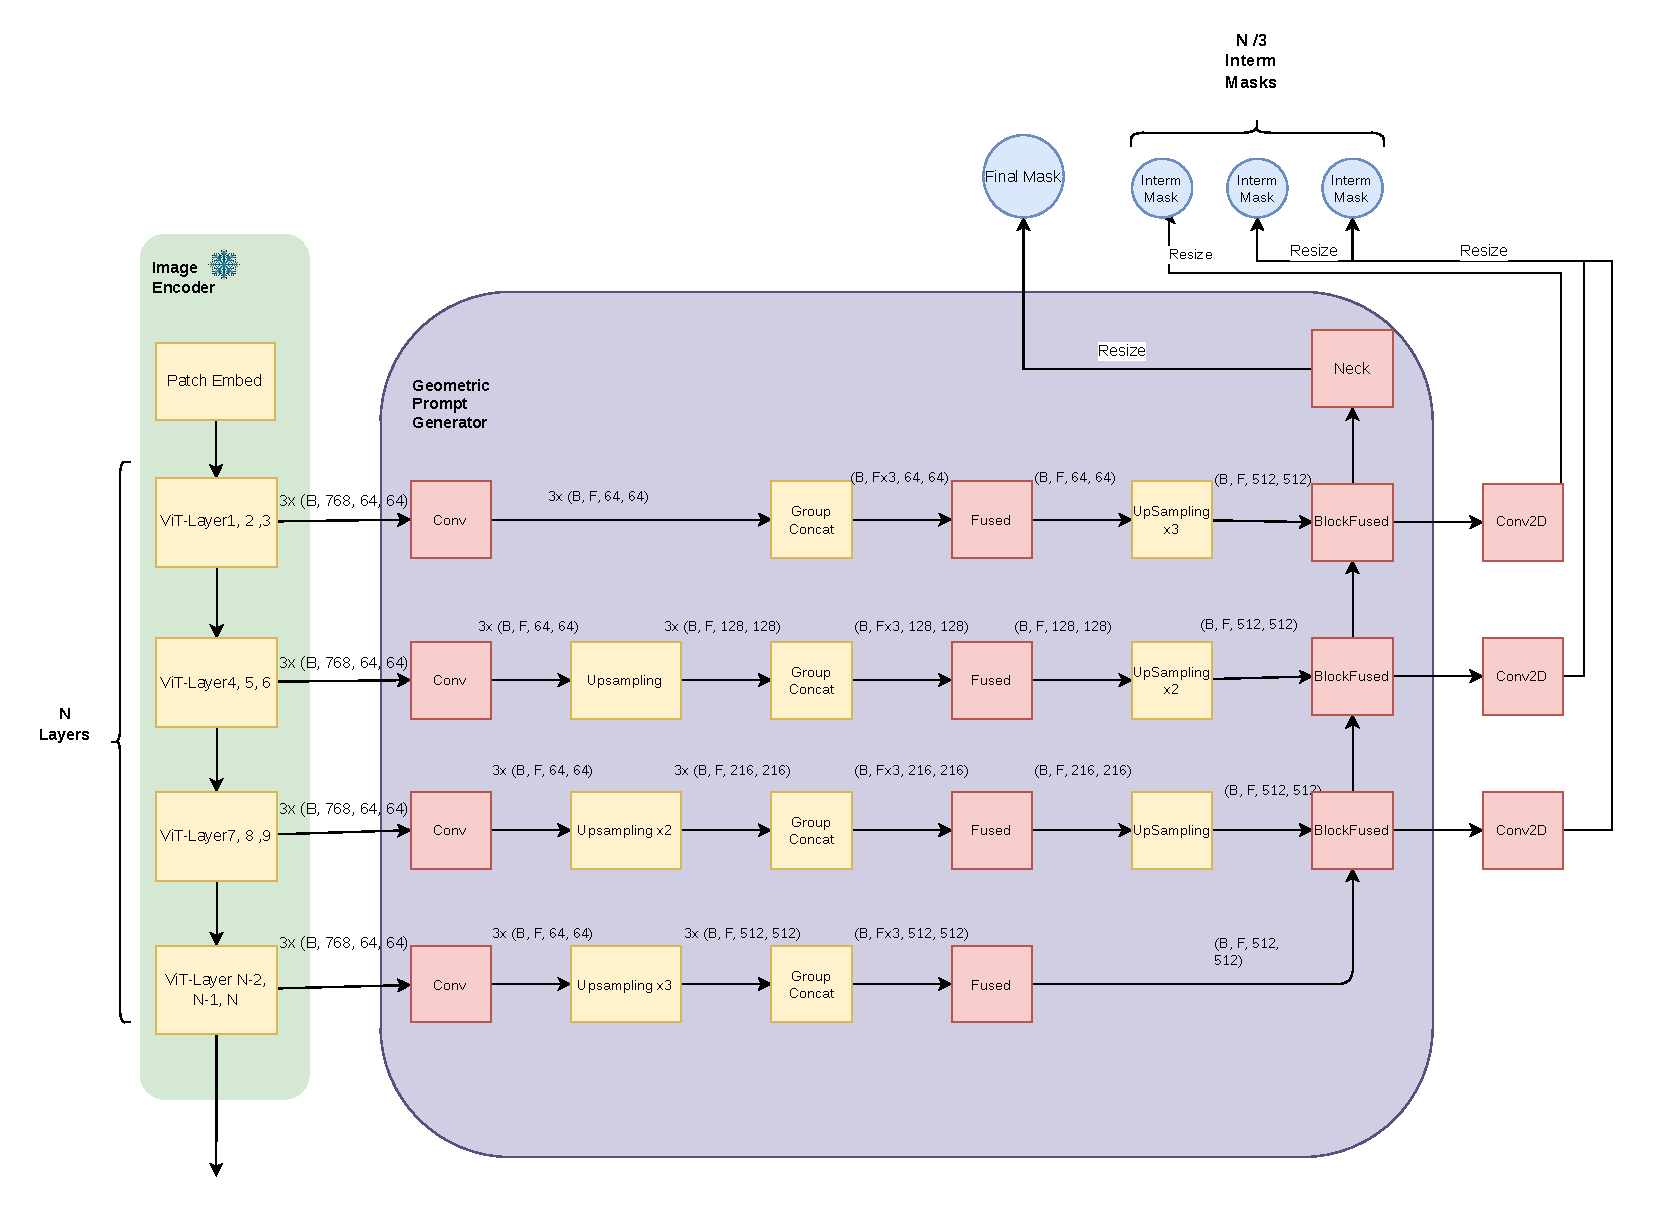
\includegraphics[width=1.2\textwidth]{graphics/approach/prompter.pdf}
    }
    \caption{Multi-scale Fusion Module}
    \label{fig:multiscalefusion}
\end{figure}